\chapter{Introducción específica} % Main chapter title

\label{Chapter2}

En este capítulo se explica en detalle el funcionamiento de un motor de combustión interna y se describe el sistema de desarrollado, sus partes y la interacción entre ellas. Al final enlista las historias de usuario y requerimientos del proyecto.

\section{Funcionamiento de un motor de combustión interna} \label{func-motor}

En la actualidad, el motor de combustión interna es el motor más utilizado en vehículos de transporte de cargas y pasajeros. Existen distintos tipos de motores que utilizan distintos tipos de combustibles. En esta sección se explicará específicamente sobre el funcionamiento de motores de pistón a gasolina.

\subsection{Proceso de combustión y su eficiencia}

Un motor de combustión interna, o motor a explosión, es un tipo de máquina que obtiene energía mecánica a través de una reacción química conocida como combustión. La combustión es la oxidación rápida en presencia de oxígeno de materiales llamados combustibles. El resultado de esta reacción, cuando la reacción es completa es, dióxido de carbono, agua, y energía liberada en forma de calor y expansión gaseosa. Es la energía liberada en forma de expansión gaseosa que es convertida en energía mecánica, y la energía liberada en forma de calor es disipada a la atmósfera. Cuando la combustión no es completa, ya sea por exceso o defecto de oxígeno, se producen otros compuestos parcialmente oxidados como el monóxido de carbono, cuando esto sucede la cantidad total de energía liberada es menor.

Para que una combustión sea completa se tiene que cumplir la condición de que la proporción por peso de oxígeno y combustible sea igual a su proporción estequiométrica. En un motor de gasolina esta proporción es de 14,7 partes de oxígeno por 1 parte de combustible\citep{book-afr}. Se le llama factor lambda, denominado con la letra griega $\lambda$, a la relación entre la proporción oxígeno y combustible actual con su proporción estequiométrica. Si la combustión ocurre con exceso de oxígeno el factor lambda será mayor a 1, si ocurre con defecto de oxígeno el factor será menor a 1, y si ocurre con la proporción justa será igual a 1. Los sensores desarrollados para poder monitorear este factor son llamados sondas lambda. En los vehículos actuales, el monitoreo de este factor es utilizado para regular la cantidad de combustible inyectada en cada proceso de combustión, de esa forma es posible operar al motor de forma eficiente minimizando las emisiones de gases indeseados.

Otra variable que afecta a la cantidad de combustible inyectada es la temperatura de los gases de admisión. La densidad de un gas depende de su temperatura y, como el volumen de la cámara de combustión es fijo, es posible calcular el peso total de oxígeno que puede caber dentro de la cámara y por lo tanto define la cantidad máxima de combustible que puede inyectarse. A menor temperatura del gas, su densidad aumenta y por lo tanto la cantidad de combustible que puede inyectarse para alcanzar la relación estequiométrica es mayor. Pero si la temperatura del gas es alta, la cantidad de combustible que puede inyectarse es menor y a menor cantidad de combustible la energía total entregada es menor.

\subsection{Eficiencia mecánica y lubricación}

Sólo una parte de la energía mecánica proveniente del proceso de combustión es convertida en energía cinética. Parte de esa energía se pierde por la fricción entre las partes móbiles que componen al motor. Para disminuir esta fricción se utilizan fluidos lubricantes, que funcionan impidiendo el contacto entre dos partes móbiles. La fricción entre las partes móbiles y el lubricante será menor que la fricción si las partes estuvieran en contacto, y al disminuir la fricción la energía perdida es menor. Para que el lubricante funcione adecuadamente su viscosidad tiene que estar dentro de un rango definido por el fabricante del motor, la misma es dependiente de la temperatura y por eso es importante monitorearla\cite{lubrication}. La temperatura de operación de un lubricante es indicada por su fabricante y su viscosidad es garantizada sólo dentro de ese margen de operación.

El lubricante es distribuido a las partes móbiles del motor a través de un circuito hidraulico cerrado. Este circuito consiste de conductos, un tanque de almacenamiento y una bomba hidraulica. La operación de esta bomba garantiza la renovación del lubricante ya que parte del lubricante se pierde por el movimiento de las partes del motor y tiene que ser recolectado y devuelto al tanque de almacenamiento. Una presión hidraúlica insuficiente puede ocasionar daños en el motor por falta de lubricación. Por eso la presión de aceite es monitoreada junto con la temperatura.

\section{Descripción general del sistema}

El sistema desarrolado consiste de dos partes distintas, la adquisidora de datos y la interfaz gráfica. La primer parte consiste de un circuito controlador por microprocesador montado cerca del motor del vehículo. El adquisidor digitaliza las señales producidas por los sensores de: temperatura de gases de admisión y escape; temperatura de aceite; sonda lambda; velocidad de giro; y tensión de la batería. Los sensores fueron seleccionados según el funcionamiento del motor explicado en \ref{func-motor}.  La información capturada por la parte adquisidora es transmitida a la segunda parte del sistema por \textit{Bluetooth Low-Energy}.

La interfaz está compuesta por una \textit{Single Board Computer} una pantalla LCD táctil y una tarjeta SD para almacenar los datos recibidos o puede ser un dispositivo móvil como un \textit{Smartphone} o \textit{Tablet}.

La figura \ref{fig:diagrama-de-bloques} es una representación en diagrama de bloques del sistema.

\begin{figure}
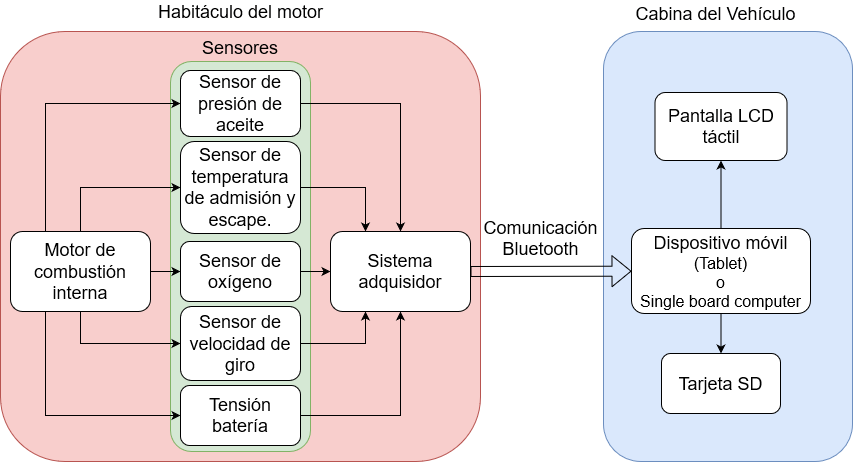
\includegraphics[width=.9\textwidth]{./Figures/diagrama-proyecto.png}
\caption{Diagrama en bloques del sistema.}
\label{fig:diagrama-de-bloques}
\end{figure}

\section{Historias de usuario y requerimientos}

El desarrollo del trabajo final fue basado en las historias de usuario y los requerimientos fijados durante la etapa de planificación del proyecto.

\subsection{Historias de usuario}\label{historias-usuario}

En la planificación del proyecto, se obtuvieron historias de usuario según un cliente interesado en instalar este dispositivo en su vehículo antiguo. Las historias compiladas son las siguientes:

\begin{itemize}
\item Como cliente quiero poder visualizar en una pantalla la información de los sensores en tiempo real en un mismo gráfico lineal para poder ver la evolución de las variables de los sensores.
\item Como cliente quiero poder definir la escala del eje temporal del gráfico lineal, y elegir entre cinco valores distintos. (1, 10, 30, 60 y 120 minutos por división) para poder ver con detalle fenómenos de corta y larga duración
\item Como cliente quiero poder elegir qué sensores deben ser mostrados en pantalla y cuáles no, para poder darle prioridad a la información que es más relevante en ese momento.
\item Como cliente quiero poder definir niveles para cada sensor individualmente y que suene una alarma cuando algún valor supere dicho nivel para ser notificado al instante de que algo no funciona adecuadamente.
\item Como cliente quiero poder descargar toda la información recolectada en una tarjeta SD o pendrive, para poder analizarla en otro momento.
\item Como cliente quiero que el sistema conmience a funcionar cuando se le da contacto al vehículo con la llave de ignición para poder ver en pantalla como funciona el motor durante el arranque.
\end{itemize}

\subsection{Requerimientos}

A partir de las historias de usuario listadas en la sección \ref{historias-usuario} se crearon los requerimientos del proyecto detallados más adelante. Los requisitos se divieron en cuatro grupos: Requerimientos generales del proyecto; requerimientos de la interfáz gráfica; requerimientos de la parte adquisidora de datos y requerimientos de la comunicación entre las partes.

Los requerimientos generales del proyecto son:
\begin{itemize}
\item REQ-GEN-001: Todo el código fuente del proyecto será almacenado bajo un sistema de control de versiones GIT.
\item REQ-GEN-002: La documentación del código fuente del sfotware embebidos será llevada a cabo en los comentarios, siguiendo el formato de Doxygen.
\item REQ-GEN-003: La documentación del software para la interfaz gráfica también será llevada a cabo en los comentarios. El formato será elegido por el responsable del proyecto.
\end{itemize}

Requerimientos de la interfáz gráfica:
\begin{itemize}
\item REQ-GUI-001: la interfaz gráfica deberá poder mostrar figuras con la información de todos los sensores a la vez.
\item REQ-GUI-002: el usuario tiene que poder elegir qué sensores ver al mismo tiempo y cuáles no desea ver.
\item REQ-GUI-003: el usuario tiene que poder definir alarmas por valor máximo, para cada una de las variables.
\item REQ-GUI-004: las alarmas serán sonores y visuales. El estilo de las alarmas será definido por el cliente durante el proceso de desarrollo de la interfáz gráfica.
\end{itemize}

Requerimientos de la parte adquisidora:
\begin{itemize}
\item REQ-ADQ-001: el sistema tiene que adquirir la temperatura de los gases de admisión y escape, con un rango de temperatura entre 0 \degree C y 400 \degree C y con una resolución menor igual a 0,5 \degree C. Con una tasa de muestreo mayor o igual a 1 hz.
\item REQ-ADQ-002: el sistema tiene que adquirir la temperatura del aceite del motor, con un rango de temperatura entre 0 \degree C y 400 \degree C y una resolución menor igual a 0,5 \degree C. Con una tasa de muestreo mayor igual a 1 hz.
\item REQ-ADQ-003: el sistema tiene que adquirir la velocidad de giro del motor, en un rango entre 0 y 20.000 revoluciones por minuto, con una resolución menor igual a 500 r.p.m. Con una tasa de muestreo mayor igual a 5 hz.
\item REQ-ADQ-004: el sistema tiene que adquirir la proporción de oxígeno en los gases de escape llamada lambda, con un rango de 0 a 2 y una resolución menor igual a 0,1 lambda.
\item REQ-ADQ-005: el sistema tiene que adquirir la presión de aceite del motor, con un rango de 0 a 100 psi y con una resolución menor igual a 1 psi.
\item REQ-ADQ-006: el sistema debe comenzar a transmitir a la interfaz gráfica la información obtenida en un tiempo no mayor a 1 segundo transcurrido el proceso de adquisición.
\end{itemize}

Requerimientos de la comunicación entre las partes del sistema:
\begin{itemize}
\item REQ-COMM-001: se permitirá que se pierda hasta 1 paquete de cada 100 paquetes transmitidos.
\end{itemize}